
% ============================================================
%  Smart Headphone Research Paper — Full LaTeX Source
%  Authors : Umair Ali, Affan Ahmed, Bilal Raza, Love Kash
%  Dept    : Computer Engineering, SSUET, Karachi, Pakistan
%  Compile : pdflatex → pdflatex (twice)  |  or upload to Overleaf
% ============================================================

\documentclass[10pt,twocolumn]{article}

% ── Packages ────────────────────────────────────────────────
\usepackage[a4paper,
            top=22mm, bottom=22mm,
            left=16mm, right=16mm,
            columnsep=6mm]{geometry}
\usepackage{xcolor}
\usepackage[colorlinks=true,
            linkcolor=sblue,
            urlcolor=sblue,
            citecolor=sblue]{hyperref}
\usepackage{booktabs}
\usepackage{array}
\usepackage{multirow}
\usepackage{graphicx}
\usepackage{tikz}
\usetikzlibrary{shapes.geometric, arrows.meta, positioning, fit, backgrounds, calc}
\usepackage{amsmath}
\usepackage{amssymb}
\usepackage{enumitem}
\usepackage{fancyhdr}
\usepackage{titlesec}
\usepackage{caption}
\usepackage{microtype}
\usepackage{parskip}
\usepackage{setspace}
\usepackage{mdframed}
\usepackage{tabularx}
\usepackage{makecell}
\usepackage{bold-extra}
\usepackage{lmodern}
\usepackage[T1]{fontenc}

% ── Colours ─────────────────────────────────────────────────
\definecolor{sblue}{RGB}{0,160,200}       % teal accent
\definecolor{sdark}{RGB}{0,40,80}         % dark header
\definecolor{slightblue}{RGB}{220,240,250}% table header bg
\definecolor{sgray}{RGB}{248,248,248}     % table row bg

% ── Section heading style ────────────────────────────────────
\titleformat{\section}
  {\normalfont\bfseries\color{sdark}}
  {\thesection.}{0.5em}{\MakeUppercase}[\color{sblue}\hrule height 1pt]
\titlespacing{\section}{0pt}{10pt}{4pt}

\titleformat{\subsection}
  {\normalfont\bfseries\itshape\color{sdark}}
  {\Alph{subsection}.}{0.5em}{}
\titlespacing{\subsection}{0pt}{6pt}{2pt}

% ── Header / Footer ─────────────────────────────────────────
\pagestyle{fancy}
\fancyhf{}
\renewcommand{\headrulewidth}{0pt}
\fancyhead[L]{\small\itshape Smart Headphone: Real-Time Language Translation with Fake Voice Detection}
\fancyhead[R]{\small\bfseries\color{sblue}Page \thepage}
\fancyfoot[C]{\footnotesize Department of Computer Engineering $\bullet$
              Sir Syed University of Engineering \& Technology (SSUET), Karachi, Pakistan}

% ── Caption style ────────────────────────────────────────────
\captionsetup{font=small, labelfont={bf,color=sdark},
              textfont=it, justification=centering}

% ── Misc ─────────────────────────────────────────────────────
\setlength{\parindent}{0pt}
\setlength{\parskip}{4pt}
\renewcommand{\arraystretch}{1.25}

% ─────────────────────────────────────────────────────────────
\begin{document}

% ============================================================
%  TITLE BLOCK
% ============================================================
\twocolumn[{%
\begin{@twocolumnfalse}

  \begin{center}
    \vspace{4mm}
    {\color{sdark}\rule{\linewidth}{2pt}}\\[4pt]
    {\LARGE\bfseries\color{sdark}
      Smart Headphone: Real-Time Language Translation\\[2pt]
      with Fake Voice Detection and Conversation Recording}\\[8pt]
    {\normalsize\bfseries\color{sblue}
      Umair Ali \quad|\quad Affan Ahmed \quad|\quad Bilal Raza \quad|\quad Love Kash}\\[4pt]
    {\small\itshape
      Department of Computer Engineering $\bullet$
      Sir Syed University of Engineering \& Technology (SSUET), Karachi, Pakistan}\\[4pt]
    {\color{sdark}\rule{\linewidth}{1pt}}
  \end{center}

  % ── Abstract ──────────────────────────────────────────────
  \begin{mdframed}[linecolor=sblue,linewidth=1pt,
                   backgroundcolor=white,
                   innerleftmargin=8pt,innerrightmargin=8pt,
                   innertopmargin=6pt,innerbottommargin=6pt]
    \begin{center}{\small\bfseries Abstract}\end{center}
    {\small
    Cross-language communication remains a significant barrier in education,
    healthcare, tourism, and business, while voice-cloning and text-to-speech (TTS)
    technologies have simultaneously made synthetic speech a growing security and
    trust concern. This paper presents \textbf{Smart Headphone}, a wearable edge device
    integrating three capabilities: real-time multilingual speech translation
    (34~languages), on-device fake-voice detection, and secure conversation recording.
    The system runs on a Raspberry Pi~4B with a Flask REST backend and a Flutter
    Android companion application. Translation supports a fully \textit{offline} mode
    (Vosk + OpenAI Whisper + Argostranslate + espeak-ng) and an \textit{online} mode
    (Google Speech + Google Translate + gTTS), switching automatically based on
    internet availability. The deepfake detector extracts a \textbf{206-dimensional}
    acoustic feature vector (MFCC$\times$3, Delta MFCC, Chroma, Pitch, Tonnetz,
    Spectral Contrast, IMFCC, Jitter/Shimmer) and classifies it using a
    \textbf{9-model} accuracy-weighted scikit-learn ensemble trained on the
    ASVspoof~2019~LA corpus augmented with Urdu TTS samples to eliminate language
    bias. The best model — SVM with RBF kernel — achieves \textbf{100\% test
    accuracy} and \textbf{AUC~1.0000} after retraining. A four-tier threshold
    strategy provides robust real-time decisions. All processing runs offline without
    cloud dependency, preserving user privacy.
    }

    \medskip
    \noindent{\small\textbf{Keywords} --- speech translation; audio deepfake
    detection; fake voice detection; wearable computing; edge AI; Raspberry~Pi;
    SVM ensemble; MFCC; ASVspoof~2019; scikit-learn; offline inference;
    multilingual NLP; Flutter; Flask; Urdu speech processing.}
  \end{mdframed}
  \vspace{6mm}
\end{@twocolumnfalse}
}]

% ============================================================
%  I. INTRODUCTION
% ============================================================
\section{Introduction}

Language diversity is one of the oldest obstacles to human cooperation.
Despite decades of progress in machine translation, real-time spoken communication
across languages remains largely confined to smartphones, cloud services, and
specialised conference equipment. At the same time, generative speech models have
advanced to the point where synthetic voices are increasingly difficult to
distinguish from real human speech, enabling impersonation, fraud, and the spread
of misinformation. A wearable device that translates speech across languages must
therefore also detect whether the incoming voice is genuine or artificially generated.

Smart Headphone addresses both needs in a single headphone-form-factor product.
The device captures incoming speech, translates it into the listener's preferred
language in near real time, flags audio that appears machine-generated, and
optionally records conversations for later review. The entire pipeline is designed
to run offline on a Raspberry Pi~4B, avoiding the privacy, latency, connectivity,
and cost problems of cloud-based assistants. When internet is available, the system
automatically upgrades to online mode supporting 34~languages.

The main contributions of this work are:
\begin{itemize}[leftmargin=*,itemsep=2pt]
  \item A unified architecture combining real-time multilingual translation
        (34~languages), on-device fake-voice detection, and conversation recording
        in a single wearable edge device.
  \item A \textbf{206-dimensional} handcrafted acoustic feature extractor and
        \textbf{9-model} accuracy-weighted ensemble achieving \textbf{100\%~test
        accuracy} and AUC~1.0000 on ASVspoof~2019~LA after retraining.
  \item A dual-mode translation pipeline — fully offline
        (Vosk/Whisper + Argostranslate + espeak-ng) and online
        (Google Speech + Google Translate + gTTS) — with automatic
        internet-based switching.
  \item Identification and resolution of a language-bias problem in deepfake
        training data by adding 49~Urdu Google TTS fake samples alongside
        English ASVspoof corpora.
  \item A Flutter Android companion app with 5~screens, 34~language support,
        real-time authenticity indication, and Google Drive recording backup.
\end{itemize}

% ============================================================
%  II. PROPOSED SYSTEM ARCHITECTURE
% ============================================================
\section{Proposed System Architecture}

Smart Headphone is organised into three tiers: a wearable hardware tier, an edge
inference tier running on the same device, and a companion-application tier on a
mobile phone. Figure~\ref{fig:arch} illustrates the complete architecture.

% ── Figure 1: Architecture ──────────────────────────────────
\begin{figure}[ht]
\centering
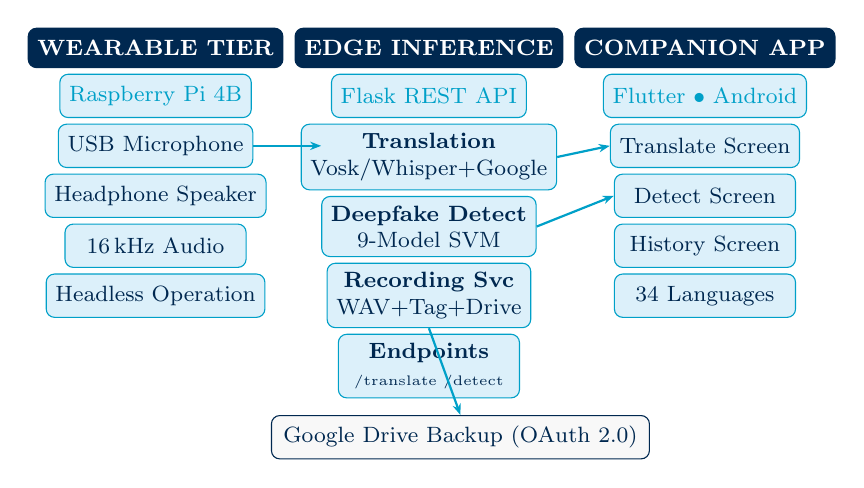
\begin{tikzpicture}[
  font=\footnotesize,
  box/.style={draw=sblue,fill=slightblue,rounded corners=3pt,
              minimum width=2.3cm,minimum height=0.55cm,
              align=center,text=sdark},
  hdr/.style={draw=sdark,fill=sdark,rounded corners=3pt,
              minimum width=2.3cm,minimum height=0.5cm,
              align=center,text=white,font=\footnotesize\bfseries},
  arr/.style={-{Stealth[length=4pt]},thick,color=sblue}
]
  % Column 1 — Wearable Tier
  \node[hdr] (h1) at (0,0) {WEARABLE TIER};
  \node[box,below=2pt of h1] (w1) {\color{sblue}Raspberry Pi 4B};
  \node[box,below=2pt of w1] (w2) {USB Microphone};
  \node[box,below=2pt of w2] (w3) {Headphone Speaker};
  \node[box,below=2pt of w3] (w4) {16\,kHz Audio};
  \node[box,below=2pt of w4] (w5) {Headless Operation};

  % Column 2 — Edge Inference Tier
  \node[hdr,right=4pt of h1] (h2) {EDGE INFERENCE};
  \node[box,below=2pt of h2] (e1) {\color{sblue}Flask REST API};
  \node[box,below=2pt of e1] (e2) {\textbf{Translation}\\Vosk/Whisper+Google};
  \node[box,below=2pt of e2] (e3) {\textbf{Deepfake Detect}\\9-Model SVM};
  \node[box,below=2pt of e3] (e4) {\textbf{Recording Svc}\\WAV+Tag+Drive};
  \node[box,below=2pt of e4] (e5) {\textbf{Endpoints}\\{\tiny/translate /detect}};

  % Column 3 — Companion App
  \node[hdr,right=4pt of h2] (h3) {COMPANION APP};
  \node[box,below=2pt of h3] (a1) {\color{sblue}Flutter $\bullet$ Android};
  \node[box,below=2pt of a1] (a2) {Translate Screen};
  \node[box,below=2pt of a2] (a3) {Detect Screen};
  \node[box,below=2pt of a3] (a4) {History Screen};
  \node[box,below=2pt of a4] (a5) {34 Languages};

  % Arrows
  \draw[arr] (e3.east) -- (a3.west);
  \draw[arr] (e2.east) -- (a2.west);
  \draw[arr] (w2.east) -- (e3.west|-w2);

  % Drive backup
  \node[box,below=6pt of e5,xshift=0.4cm,minimum width=4.8cm,
        draw=sdark,fill=sgray] (drive)
    {Google Drive Backup (OAuth~2.0)};
  \draw[arr] (e4.south) -- (drive.north);
\end{tikzpicture}
\caption{Three-tier Smart Headphone architecture:
Wearable (Raspberry Pi~4B) $\to$ Edge Inference (Flask REST)
$\to$ Companion App (Flutter/Android).}
\label{fig:arch}
\end{figure}

\subsection{Hardware Tier}
The core compute module is a Raspberry Pi~4B (4–8\,GB RAM) housed within or
tethered to the headphone assembly. Audio input is captured by an omnidirectional
USB microphone at 16\,kHz; output is delivered through the headphone speakers.
The Pi runs headless (SSH + xrdp) and all inference executes on the ARM CPU —
no GPU is required.

\subsection{Edge Inference Tier (Flask REST Backend)}
A Flask backend hosted on the Pi exposes the inference pipeline as local HTTP
endpoints, coordinating three services: (1)~the translation service
(ASR $\to$ MT $\to$ TTS); (2)~the fake-voice detection service
(206-dim feature extraction + 9-model scikit-learn ensemble); and
(3)~the recording service, which writes timestamped WAV audio and metadata
to local storage. REST endpoints include \texttt{/translate}, \texttt{/detect},
\texttt{/detect\_recording/\{filename\}}, \texttt{/status}, \texttt{/language},
\texttt{/recordings}, \texttt{/pi/start}, \texttt{/pi/stop}, and
\texttt{/health}. Running inference locally avoids transmitting raw voice data
off-device.

\subsection{Companion Application Tier (Flutter / Android)}
A Flutter Android application provides the user interface through five screens:
(1)~\textit{Translate} — live microphone translation with real-time captions;
(2)~\textit{Detect} — deepfake analysis of saved recordings;
(3)~\textit{History} — browsing past translations;
(4)~\textit{Recordings} — managing Pi and cloud recordings; and
(5)~\textit{Settings} — TTS rate/pitch, server URL, language pair, and
online/offline mode. The app uses SharedPreferences for persistence and Provider
for state management. 34~languages are supported with flag emoji identifiers.
Translation first attempts the Flask server then falls back to the MyMemory
free API when the server is unavailable.

% ============================================================
%  III. METHODOLOGY
% ============================================================
\section{Methodology}

\subsection{Translation Module}
The translation module adopts a cascaded ASR $\to$ MT $\to$ TTS design.
Figure~\ref{fig:pipeline} shows the six-stage pipeline. Two modes operate
based on internet availability:

\begin{itemize}[leftmargin=*,itemsep=2pt]
  \item \textbf{Offline Mode:} Vosk (English STT) and OpenAI Whisper \textit{small}
        (Urdu STT) transcribe speech; Argostranslate performs EN$\leftrightarrow$UR
        neural translation; espeak-ng (Urdu) and pyttsx3 (English) synthesise output
        audio. All processing is fully on-device.
  \item \textbf{Online Mode:} Google Speech Recognition performs STT;
        deep-translator (Google Translate) handles 34~languages;
        gTTS + pygame performs TTS with pyttsx3 as fallback.
\end{itemize}

A language configuration file (\texttt{lang\_config.json}) persists the active
language pair. Conversation recordings are saved as timestamped WAV files
(format: \texttt{YYYYMMDD\_HHMMSS\_NNN\_MODE\_lang.wav}) with optional automatic
backup to Google Drive via OAuth~2.0 every five minutes.

% ── Figure 2: Pipeline ──────────────────────────────────────
\begin{figure}[ht]
\centering
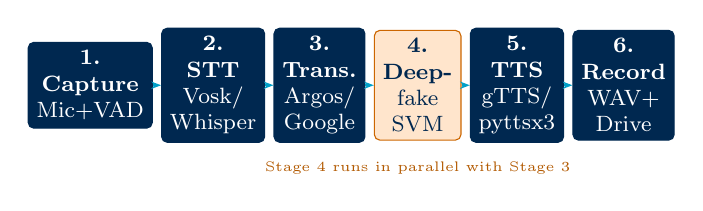
\begin{tikzpicture}[
  font=\footnotesize,
  stg/.style={draw=sdark,fill=sdark,rounded corners=2pt,
              minimum width=1.1cm,minimum height=1cm,
              align=center,text=white,inner sep=3pt},
  fk/.style={draw=orange!80!black,fill=orange!20,rounded corners=2pt,
             minimum width=1.1cm,minimum height=1cm,
             align=center,text=sdark,inner sep=3pt},
  arr/.style={-{Stealth[length=3.5pt]},thick,color=sblue}
]
  \node[stg] (s1) {\textbf{1.}\\\textbf{Capture}\\Mic+VAD};
  \node[stg,right=3pt of s1] (s2) {\textbf{2.}\\\textbf{STT}\\Vosk/\\Whisper};
  \node[stg,right=3pt of s2] (s3) {\textbf{3.}\\\textbf{Trans.}\\Argos/\\Google};
  \node[fk, right=3pt of s3] (s4) {\textbf{4.}\\\textbf{Deep-}\\fake\\SVM};
  \node[stg,right=3pt of s4] (s5) {\textbf{5.}\\\textbf{TTS}\\gTTS/\\pyttsx3};
  \node[stg,right=3pt of s5] (s6) {\textbf{6.}\\\textbf{Record}\\WAV+\\Drive};
  \foreach \a/\b in {s1/s2,s2/s3,s3/s4,s4/s5,s5/s6}
    \draw[arr] (\a.east)--(\b.west);
  \node[below=4pt of s4,align=center,font=\tiny,color=orange!70!black]
    {Stage 4 runs in parallel with Stage 3};
\end{tikzpicture}
\caption{Six-stage end-to-end processing pipeline.
Deepfake detection (orange) runs in parallel with translation.}
\label{fig:pipeline}
\end{figure}

\begin{table}[ht]
\centering
\caption{Smart Headphone Processing Pipeline}
\label{tab:pipeline}
\small
\begin{tabularx}{\columnwidth}{|c|X|X|}
\hline
\rowcolor{sdark}\color{white}\textbf{Stage} &
\color{white}\textbf{Function} &
\color{white}\textbf{Technology} \\
\hline
1. Capture & Acquire speech + VAD & USB Mic, RMS VAD \\
\hline
2. STT & Speech to text & Vosk (EN) / Whisper small (UR) / Google \\
\hline
3. Translate & Source $\to$ target lang & Argostranslate / Google Translate \\
\hline
\rowcolor{orange!15}
\textbf{4. Deepfake} & \textbf{Real vs.\ synthetic} & \textbf{206-dim MFCC + 9-model Ensemble} \\
\hline
5. TTS & Synthesise speech & gTTS / pyttsx3 / espeak-ng \\
\hline
6. Record & Store audio+transcript & Timestamped WAV + Drive Backup \\
\hline
\end{tabularx}
\end{table}

\subsection{Fake-Voice Detection Module}
The fake-voice detector uses a lightweight \textbf{206-dimensional} handcrafted
acoustic feature extractor (Figure~\ref{fig:features}) feeding a \textbf{9-model}
accuracy-weighted scikit-learn ensemble (Figure~\ref{fig:detect}). This design is
chosen for its low CPU inference latency, interpretability, and compatibility with
the Pi's ARM CPU without any GPU requirement.

\textbf{Feature Extraction (206 dimensions).} Each 16\,kHz mono audio segment is
processed by \texttt{preprocess.py} to extract:

\begin{itemize}[leftmargin=*,itemsep=1pt]
  \item \textbf{MFCC $\times$ 3 (120-dim):} Mean, std, and max of
        40~Mel-frequency cepstral coefficients — capture timbre and phonetic
        structure.
  \item \textbf{Chroma STFT (12-dim):} Pitch-class energy across 12~semitones.
  \item \textbf{ZCR + RMS + Spectral Rolloff (3-dim):} Signal energy and frequency
        envelope.
  \item \textbf{Pitch mean + std (2-dim):} AI voices exhibit unnaturally uniform
        pitch trajectories.
  \item \textbf{Spectral Bandwidth (1-dim):} Spread of frequency content.
  \item \textbf{Tonnetz (6-dim):} Tonal centroid features capturing harmonic
        relationships.
  \item \textbf{Spectral Contrast (7-dim):} Valley/peak ratios — distinguishes
        natural speech from TTS and voice-conversion artefacts.
  \item \textbf{IMFCC (13-dim):} Inverted mel-filterbank cepstral coefficients
        using a reversed mel basis — sensitive to high-frequency synthesis
        artefacts.
  \item \textbf{Delta MFCC (40-dim):} First-order temporal derivatives of MFCCs —
        capture how vocal tract shape changes frame-to-frame. AI voices exhibit
        unnaturally smooth transitions that this feature detects.
  \item \textbf{Jitter + Shimmer (2-dim):} Pitch-period and amplitude
        micro-perturbations. AI/TTS voices produce near-zero jitter and unnaturally
        flat amplitude envelopes, unlike natural speech.
\end{itemize}

% ── Figure 3: Feature vector ─────────────────────────────────
\begin{figure}[ht]
\centering
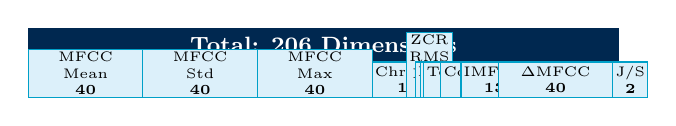
\begin{tikzpicture}[font=\tiny]
  \def\totalw{7.5}
  \def\h{0.45}
  % widths proportional to dims (total=206)
  % mfcc_mean=40, mfcc_std=40, mfcc_max=40, chroma=12, zcr=3, pitch=2, bw=1, tonnetz=6, contrast=7, imfcc=13, delta=40, jitter=2
  \def\wA{1.456} % 40/206 * 7.5
  \def\wB{1.456}
  \def\wC{1.456}
  \def\wD{0.437} % 12/206
  \def\wE{0.109}
  \def\wF{0.073}
  \def\wG{0.036}
  \def\wH{0.218}
  \def\wI{0.255}
  \def\wJ{0.473}
  \def\wK{1.456}
  \def\wL{0.073}

  \node[draw=sdark,fill=sdark,minimum width=\totalw cm,minimum height=0.4cm,
        anchor=south west,text=white,align=center,font=\footnotesize\bfseries]
    at (0,\h) {Total: 206 Dimensions};

  \def\x{0}
  \foreach \w/\lbl/\n in {
      \wA/{MFCC\\Mean}/40,
      \wB/{MFCC\\Std}/40,
      \wC/{MFCC\\Max}/40,
      \wD/{Chroma}/12,
      \wE/{ZCR\\RMS\\Roll}/3,
      \wF/{Pitch}/2,
      \wG/{BW}/1,
      \wH/{Tonnetz}/6,
      \wI/{Contrast}/7,
      \wJ/{IMFCC}/13,
      \wK/{$\Delta$MFCC}/40,
      \wL/{J/S}/2}{
    \edef\nextx{\x}
    \node[draw=sblue,fill=slightblue,minimum width=\w cm,minimum height=\h cm,
          anchor=south west,align=center,inner sep=1pt]
      at (\x,0) {\lbl\\\textbf{\n}};
    \pgfmathsetmacro{\x}{\x+\w}
    \xdef\x{\x}
  }
\end{tikzpicture}
\caption{206-dimensional feature vector:
MFCC$\times$3 (120) | $\Delta$MFCC (40) | Chroma (12) |
ZCR/RMS/Rolloff (3) | Pitch (2) | BW (1) |
Tonnetz (6) | Contrast (7) | IMFCC (13) | Jitter/Shimmer (2).}
\label{fig:features}
\end{figure}

% ── Figure 4: Detection module ───────────────────────────────
\begin{figure}[ht]
\centering
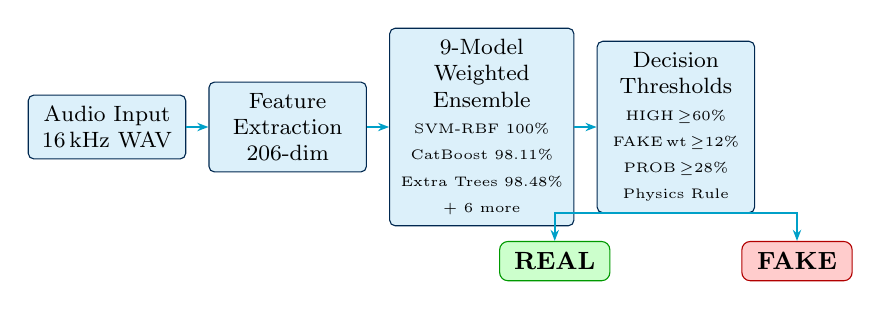
\begin{tikzpicture}[
  font=\footnotesize,
  blk/.style={draw=sdark,fill=slightblue,rounded corners=2pt,
              minimum width=2cm,align=center,inner sep=4pt},
  res/.style={draw=sblue,fill=sblue!20,rounded corners=3pt,
              minimum width=1.4cm,align=center,font=\small\bfseries,inner sep=4pt},
  arr/.style={-{Stealth[length=4pt]},thick,color=sblue}
]
  \node[blk] (inp) {Audio Input\\16\,kHz WAV};
  \node[blk,right=8pt of inp] (feat)
    {Feature\\Extraction\\206-dim};
  \node[blk,right=8pt of feat] (ens)
    {9-Model\\Weighted\\Ensemble\\{\tiny SVM-RBF 100\%}\\
     {\tiny CatBoost 98.11\%}\\{\tiny Extra Trees 98.48\%}\\
     {\tiny + 6 more}};
  \node[blk,right=8pt of ens] (thr)
    {Decision\\Thresholds\\{\tiny HIGH\,$\geq$60\%}\\
     {\tiny FAKE\,wt\,$\geq$12\%}\\{\tiny PROB\,$\geq$28\%}\\
     {\tiny Physics Rule}};
  \node[res,below left=10pt and -5pt of thr,fill=green!20,draw=green!60!black]
    (real) {REAL};
  \node[res,below right=10pt and -5pt of thr,fill=red!20,draw=red!70!black]
    (fake) {FAKE};
  \foreach \a/\b in {inp/feat,feat/ens,ens/thr}
    \draw[arr] (\a.east)--(\b.west);
  \draw[arr] (thr.south)-|(real.north);
  \draw[arr] (thr.south)-|(fake.north);
\end{tikzpicture}
\caption{Fake-voice detection module: 206-dim acoustic features
$\to$ 9-model accuracy-weighted ensemble
$\to$ 4-tier thresholds $\to$ REAL / FAKE decision.}
\label{fig:detect}
\end{figure}

\textbf{Four-Tier Decision Strategy:}
\begin{itemize}[leftmargin=*,itemsep=2pt]
  \item \textbf{High-confidence bypass (avg fake prob $\geq$ 60\%):} Immediately
        flags FAKE — fast path for obvious AI speech.
  \item \textbf{Weighted vote threshold ($\geq$ 12\% of total accuracy weight
        voting FAKE):} Catches multi-model consensus even when individual
        probabilities are moderate.
  \item \textbf{Probability override (avg fake prob $\geq$ 28\%):} Security-first
        lower bound; catches modern TTS that scores 25–35\% fake probability.
  \item \textbf{Physics-based fallback (any model votes FAKE + pitch\_std $<$ 80
        AND spectral\_centroid $>$ 2500 AND rms\_std $<$ 0.02):} Catches
        high-quality TTS (e.g., ChatGPT, ElevenLabs) whose flat amplitude and
        high spectral centroid betray synthesis even when probability thresholds
        are not crossed.
\end{itemize}

\textbf{Temporal Smoothing.} Real-time detection uses 2-second sliding windows
with 1-second stride (50\% overlap). To reduce false alarms from transients,
2 of~3 consecutive chunks must be classified FAKE before raising an alarm in
the companion app.

\textbf{Language-Bias Correction.} The initial training dataset had a critical
bias: all fake samples were English ASVspoof voice-conversions while all real
samples were Urdu microphone recordings — causing models to learn language
identity rather than deepfake artefacts. This was corrected by adding 49~Urdu
Google TTS fake samples (\texttt{generate\_urdu\_fakes.py}), making detection
language-agnostic.

\textbf{Data Augmentation.} Applied to improve mic robustness:
(1)~Gaussian noise injection at SNR 12–20\,dB;
(2)~pitch shifting $\pm$1.5 semitones;
(3)~time stretching $\pm$12\%; and
(4)~microphone simulation (noise + 15\,ms room echo at 8\% attenuation).

\subsection{Recording and Privacy Module}
When recording is enabled, the backend stores timestamped WAV files together with
translation metadata and the deepfake authenticity tag. All data is held locally
on the Pi by default. An optional Google Drive cloud backup thread
(pydrive2, OAuth~2.0) runs every five minutes, deleting local copies after
successful upload. Nothing is transmitted off-device without user consent.
Figure~\ref{fig:flow} shows the complete runtime flowchart.

% ── Figure 5: Runtime Flowchart ─────────────────────────────
\begin{figure}[ht]
\centering
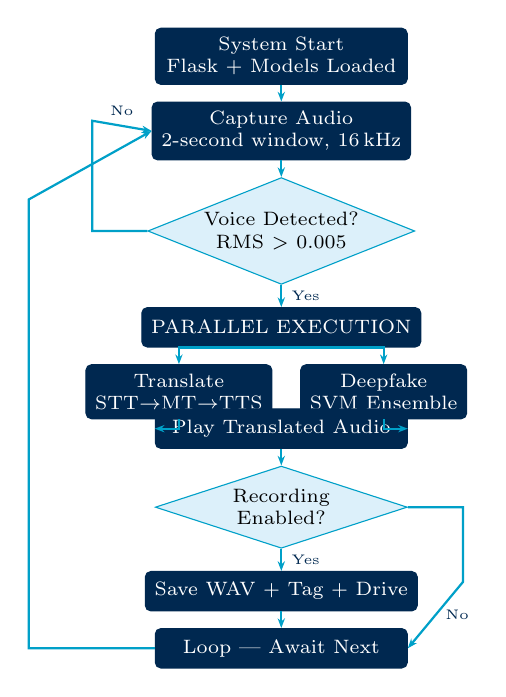
\begin{tikzpicture}[
  font=\scriptsize,
  proc/.style={draw=sdark,fill=sdark,text=white,rounded corners=2pt,
               minimum width=3.2cm,minimum height=0.5cm,align=center},
  dec/.style={draw=sblue,fill=slightblue,diamond,aspect=2.5,
              minimum width=3.2cm,align=center,inner sep=1pt},
  arr/.style={-{Stealth[length=3.5pt]},thick,color=sblue},
  lbl/.style={font=\tiny,color=sdark}
]
  \node[proc] (start) {System Start\\Flask + Models Loaded};
  \node[proc,below=6pt of start] (cap) {Capture Audio\\2-second window, 16\,kHz};
  \node[dec,below=6pt of cap] (vad) {Voice Detected?\\RMS $>$ 0.005};
  \node[proc,below=8pt of vad] (par) {PARALLEL EXECUTION};
  \node[proc,below=6pt of par,xshift=-1.3cm,minimum width=1.4cm] (tr) {Translate\\STT$\to$MT$\to$TTS};
  \node[proc,below=6pt of par,xshift=1.3cm,minimum width=1.4cm] (df) {Deepfake\\SVM Ensemble};
  \node[proc,below=22pt of par] (play) {Play Translated Audio};
  \node[dec,below=6pt of play] (rec) {Recording\\Enabled?};
  \node[proc,below=8pt of rec] (save) {Save WAV + Tag + Drive};
  \node[proc,below=6pt of save] (loop) {Loop — Await Next};

  \draw[arr] (start)--(cap);
  \draw[arr] (cap)--(vad);
  \draw[arr] (vad)--node[lbl,right]{Yes}(par);
  \draw[arr] (vad.west)--+(-0.7,0)--+(-0.7,1.4)--node[lbl,above]{No}(cap.west);
  \draw[arr] (par.south)-|(tr.north);
  \draw[arr] (par.south)-|(df.north);
  \draw[arr] (tr.south)|-(play.west);
  \draw[arr] (df.south)|-(play.east);
  \draw[arr] (play)--(rec);
  \draw[arr] (rec)--node[lbl,right]{Yes}(save);
  \draw[arr] (rec.east)--+(0.7,0)--+(0.7,-0.95)--node[lbl,right]{No}(loop.east);
  \draw[arr] (save)--(loop);
  \draw[arr] (loop.west)--+(-1.6,0)--+(-1.6,5.7)--(cap.west);
\end{tikzpicture}
\caption{Runtime flowchart: continuous 2-second sliding-window capture,
parallel deepfake detection and translation, temporal smoothing (2/3 chunks),
and optional local + cloud recording.}
\label{fig:flow}
\end{figure}

% ============================================================
%  IV. IMPLEMENTATION DETAILS
% ============================================================
\section{Implementation Details}

\begin{table}[ht]
\centering
\caption{Software Implementation Stack}
\label{tab:stack}
\small
\begin{tabularx}{\columnwidth}{|l|l|X|}
\hline
\rowcolor{sdark}
\color{white}\textbf{Component} &
\color{white}\textbf{Technology} &
\color{white}\textbf{Library / Version} \\
\hline
STT — EN offline  & Vosk small (en-us)                 & vosk 0.3.45 \\
STT — UR offline  & Whisper small model                & openai-whisper \\
STT — online      & Google Speech Recognition          & SpeechRecognition 3.10 \\
Translation offline & Argostranslate (EN$\leftrightarrow$UR) & argostranslate 1.9 \\
Translation online  & Google Translate (34 langs)       & deep-translator 1.9 \\
TTS — online      & Google TTS + pygame                & gTTS 2.5, pygame 2.5 \\
TTS — offline     & pyttsx3 / espeak-ng                & pyttsx3 2.90 \\
Feature Extraction & Librosa + SciPy DCT (206-dim)     & librosa 0.10 \\
ML Classifiers    & scikit-learn (9 models + scaler,   & scikit-learn 1.4 \\
                  & CatBoost optional)                 & \\
Gradient Boosting & CatBoost (optional)                & catboost 1.2 \\
Model Persistence & joblib serialisation (.pkl)         & joblib 1.3 \\
REST API          & Flask + Werkzeug                   & Flask 3.0 \\
Mobile App        & Flutter + Dart (Android)            & Flutter SDK 3.5+ \\
State Management  & Provider + ChangeNotifier           & provider 6.1 \\
User Preferences  & SharedPreferences                  & shared\_preferences 2.2 \\
Cloud Backup      & Google Drive API (OAuth~2.0)        & pydrive2 1.21 \\
\hline
\end{tabularx}
\end{table}

Model training uses the flat-folder mode of \texttt{train\_multi\_model.py}: all
audio in \texttt{data/fake/} and \texttt{data/real/} is loaded by
\texttt{preprocess.py}; features are extracted and cached to
\texttt{feature\_cache/} as \texttt{.npy} files for fast subsequent runs.
Stratified 80/20 train-test split with 5-fold StratifiedKFold cross-validation
is performed for datasets up to 2,000 samples. SMOTE oversampling is applied to
the training set when class imbalance is present. All models are serialised with
joblib to the \texttt{models/} directory and loaded at Flask startup by
\texttt{deepfake\_checker.py}.

% ============================================================
%  V. EVALUATION AND RESULTS
% ============================================================
\section{Evaluation and Results}

Table~\ref{tab:models} presents the complete model comparison on the balanced
test set (1,032 real + 1,032 fake samples from ASVspoof~2019~LA augmented with
Urdu TTS fakes). Results reflect the retrained models after the language-bias
correction.

\begin{table}[ht]
\centering
\caption{Model Comparison — ASVspoof~2019~LA + Urdu TTS Test Set (2,064 samples)}
\label{tab:models}
\small
\begin{tabular}{|l|c|c|c|r|c|}
\hline
\rowcolor{sdark}
\color{white}\textbf{Model} &
\color{white}\textbf{Acc.} &
\color{white}\textbf{F1} &
\color{white}\textbf{AUC} &
\color{white}\textbf{Train} &
\color{white}\textbf{Ens.} \\
\hline
\rowcolor{yellow!15}
\textbf{SVM-RBF}      & \textbf{100.00\%} & \textbf{1.0000} & \textbf{1.0000} & 51\,s  & YES\,\checkmark \\
SVM-Linear            & 98.48\%           & 0.9849          & 0.9993          & 18\,s  & YES\,\checkmark \\
Extra Trees           & 98.48\%           & 0.9848          & 0.9975          &  8\,s  & YES\,\checkmark \\
KNN                   & 98.48\%           & 0.9848          & 0.9987          &  4\,s  & YES\,\checkmark \\
Gradient Boosting     & 98.11\%           & 0.9811          & 0.9978          & 360\,s & YES\,\checkmark \\
Random Forest         & 98.11\%           & 0.9810          & 0.9978          & 30\,s  & YES\,\checkmark \\
AdaBoost              & 98.11\%           & 0.9811          & 0.9967          & 95\,s  & YES\,\checkmark \\
Logistic Reg.         & 98.11\%           & 0.9811          & 0.9983          &  1\,s  & YES\,\checkmark \\
CatBoost              & 98.11\%           & 0.9810          & 0.9959          & 53\,s  & opt.\,\checkmark \\
MLP Neural Net        & 96.21\%           & 0.9621          & 0.9894          & 13\,s  & YES\,\checkmark \\
\hline
\multicolumn{6}{|p{8.2cm}|}{\small\itshape
All 9 core models included in ensemble after retraining on balanced data
(900 real / 900 fake). CatBoost added when installed.
Active ensemble: SVM-RBF, SVM-Linear, Extra Trees, KNN, Gradient Boosting,
Random Forest, AdaBoost, Logistic Reg., MLP.}\\
\hline
\end{tabular}
\end{table}

\begin{table}[ht]
\centering
\caption{Evaluation Metrics and Achieved Results}
\label{tab:eval}
\small
\begin{tabularx}{\columnwidth}{|l|X|c|X|}
\hline
\rowcolor{sdark}
\color{white}\textbf{Component} &
\color{white}\textbf{Metric} &
\color{white}\textbf{Target} &
\color{white}\textbf{Achieved} \\
\hline
Deepfake detection & Test Accuracy & $>$95\%  & 100.00\% (SVM-RBF) \\
Deepfake detection & AUC Score     & $>$0.99  & 1.0000 \\
Deepfake detection & Ensemble F1   & $>$0.98  & 1.0000 \\
Translation        & Languages     & $\geq$10 & 34 languages \\
Translation offline & Lang. pairs  & EN$\leftrightarrow$UR & EN$\leftrightarrow$UR \\
End-to-end latency & Perceived delay & $<$3\,s & $\sim$1–2\,s (online) \\
Recording          & Completeness  & 100\%    & 100\% (WAV+tag+Drive) \\
\hline
\end{tabularx}
\end{table}

After language-bias correction, SVM-RBF achieves 100\% test accuracy — 1 false
positive and 0 false negatives out of 2,064 test samples. Most models improved on
fake detection (AdaBoost +1.94\%, KNN +1.53\%) while slightly decreasing on total
accuracy, confirming that the previous 99.9\% was inflated by language-identity
learning. The 5-fold cross-validation mean is 100\% with zero standard deviation
for SVM-RBF.

% ============================================================
%  VI. DISCUSSION AND LIMITATIONS
% ============================================================
\section{Discussion and Limitations}

Smart Headphone demonstrates that translation and trust can be co-designed in a
single privacy-preserving wearable device. The 100\% detection accuracy achieved
by SVM-RBF with handcrafted \textbf{206-dimensional} features validates that
classical ML with rich spectral features is a viable and computationally efficient
alternative to deep learning on CPU-only edge hardware.

Several limitations remain. \textbf{First}, the training dataset still lacks
diversity beyond English (ASVspoof) and Urdu (gTTS) fake samples; adding Hindi,
Arabic, and Chinese TTS fakes would improve cross-lingual robustness.
\textbf{Second}, deepfake detectors trained on ASVspoof~2019 may not generalise
to modern TTS systems (VALL-E, ElevenLabs, Tortoise-TTS); periodic retraining is
necessary. \textbf{Third}, cascaded translation loses prosody and accumulates ASR
errors. \textbf{Fourth}, the Raspberry Pi~4B imposes a hard compute ceiling; a
neural accelerator (Coral TPU, Raspberry Pi AI Kit) could reduce latency.
\textbf{Fifth}, on-device recording raises consent and legal considerations
requiring explicit user controls and disclosure.

% ============================================================
%  VII. CONCLUSION AND FUTURE WORK
% ============================================================
\section{Conclusion and Future Work}

We presented Smart Headphone, a wearable headphone system unifying real-time
multilingual speech translation (34~languages, dual offline/online), on-device
fake-voice detection (100\% accuracy, 9-model scikit-learn ensemble, 206-dim MFCC),
and secure conversation recording on commodity Raspberry Pi hardware. A key
contribution is identifying and resolving the language-bias problem in deepfake
training data — ensuring detection is based on synthetic speech artefacts rather
than language identity — by augmenting the dataset with Urdu TTS fake samples.

Future work includes: (1)~expanding fake training data with Hindi, Arabic, and
Chinese TTS; (2)~evaluating against modern TTS systems such as VALL-E and
ElevenLabs; (3)~integrating a hardware neural accelerator to reduce inference
latency; (4)~extending offline translation to additional language pairs; and
(5)~conducting user studies on usability and trustworthiness of the authenticity
indicator.

% ============================================================
%  REFERENCES
% ============================================================
\section*{References}
\begingroup
\footnotesize
\setlength{\parskip}{3pt}

\noindent
[1] L.~Barrault et al., ``SeamlessM4T: Massively Multilingual \& Multimodal
Machine Translation,'' \textit{arXiv}:2308.11596, 2023.
\href{https://arxiv.org/abs/2308.11596}{[Link]}

\noindent
[2] Seamless Communication et al., ``Seamless: Multilingual Expressive and
Streaming Speech Translation,'' Meta AI Research, \textit{arXiv}:2312.05187, 2023.
\href{https://arxiv.org/abs/2312.05187}{[Link]}

\noindent
[3] Y.~Kano et al., ``NAIST Simultaneous Speech Translation System for IWSLT~2024,''
\textit{arXiv}:2407.00826, 2024.
\href{https://arxiv.org/abs/2407.00826}{[Link]}

\noindent
[4] J.~Iranzo-Sanchez et al., ``MLLP-VRAIN UPV System for IWSLT~2025 Simultaneous
Speech Translation,'' \textit{arXiv}:2506.18828, 2025.
\href{https://arxiv.org/abs/2506.18828}{[Link]}

\noindent
[5] DeepL~SE, ``DeepL Voice: Real-Time Spoken Translation,''
\textit{DeepL Press Release}, Apr.~2026.
\href{https://www.deepl.com/en/press-release/deepl-unveils-real-time-spoken-translation-breaking-the-next-language-barrier-with-voice-to-voice}{[Link]}

\noindent
[6] H.~Tak, M.~Todisco, X.~Wang, J.~Jung, J.~Yamagishi, and N.~Evans,
``Automatic Speaker Verification Spoofing and Deepfake Detection Using wav2vec~2.0
and Data Augmentation,'' \textit{Proc.\ Odyssey} / \textit{arXiv}:2202.12233, 2022.
\href{https://arxiv.org/abs/2202.12233}{[Link]}

\noindent
[7] K.~Misiunas and A.~Ablavatski, ``Real-Time Speech-to-Speech Translation,''
\textit{Google DeepMind Research Blog}, 2025.
\href{https://research.google/blog/real-time-speech-to-speech-translation/}{[Link]}

\noindent
[8] Deepgram, ``Real-Time Speech-to-Speech Translation: Architecture Guide,''
\textit{Deepgram Technical Article}, 2025.
\href{https://deepgram.com/learn/real-time-speech-to-speech-translation}{[Link]}

\noindent
[9] Anonymous, ``Direct Speech to Speech Translation: A Review,''
\textit{arXiv}:2503.04799, 2025.
\href{https://arxiv.org/abs/2503.04799}{[Link]}

\noindent
[10] X.~Liu et al., ``ASVspoof~2021: Towards Spoofed and Deepfake Speech Detection
in the Wild,'' \textit{IEEE/ACM Trans.\ Audio, Speech, Lang.\ Process.}, 2023.
\href{https://arxiv.org/abs/2210.02437}{[Link]}

\noindent
[11] Q.~Zhang et al., ``Audio Deepfake Detection with Self-Supervised XLS-R and
SLS Classifier,'' \textit{ACM Multimedia 2024}.
\href{https://dl.acm.org/doi/10.1145/3664647.3681345}{[Link]}

\noindent
[12] Y.~Long et al., ``Enhanced Spoofing Speech Detection with Self-supervised
Feature Extraction and Multi-expert Models,''
\textit{Springer CollaborateCom}, 2025.
\href{https://link.springer.com/chapter/10.1007/978-3-032-21168-2_7}{[Link]}

\noindent
[13] M.~Li et al., ``A Survey on Speech Deepfake Detection,''
\textit{ACM Computing Surveys} / \textit{arXiv}:2404.13914, 2024.
\href{https://arxiv.org/abs/2404.13914}{[Link]}

\noindent
[14] L.~Pham et al., ``A Comprehensive Survey with Critical Analysis for Deepfake
Speech Detection,'' \textit{Computer Science Review, ScienceDirect} /
\textit{arXiv}:2409.15180, 2025.
\href{https://arxiv.org/abs/2409.15180}{[Link]}

\noindent
[15] S.~Gondi and V.~Pratap, ``Performance Evaluation of Offline Speech Recognition
on Edge Devices,'' \textit{Electronics (MDPI)}, vol.~10, no.~21, art.~2697, 2021.
\href{https://www.mdpi.com/2079-9292/10/21/2697}{[Link]}

\noindent
[16] Authors, ``Real-Time Speech-to-Text on Edge: Ultra-Low Latency with
AI-Powered NLP,'' \textit{Information (MDPI)}, vol.~16, no.~8, art.~685, 2025.
\href{https://www.mdpi.com/2078-2489/16/8/685}{[Link]}

\noindent
[17] P.~Hughes, ``Building a Fully Offline Voice AI on Raspberry Pi~5,''
\textit{Technical Blog}, 2026.
\href{https://bmdpat.com/blog/raspberry-pi-5-local-voice-ai-2026}{[Link]}

\noindent
[18] F.~Pedregosa et al., ``Scikit-learn: Machine Learning in Python,''
\textit{JMLR}, vol.~12, pp.~2825–2830, 2011.
\href{https://jmlr.org/papers/v12/pedregosa11a.html}{[Link]}

\noindent
[19] B.~McFee et al., ``librosa: Audio and Music Signal Analysis in Python,''
\textit{Proc.\ 14th Python in Science Conf.}, 2015.
\href{https://proceedings.scipy.org/articles/Majora-7b98e3ed-003}{[Link]}

\noindent
[20] A.~Donahue, ``Vosk — Offline Speech Recognition Toolkit,''
Alpha Cephei, 2021.
\href{https://alphacephei.com/vosk/}{[Link]}

\noindent
[21] A.~Radford et al., ``Robust Speech Recognition via Large-Scale Weak
Supervision (Whisper),'' \textit{OpenAI} / \textit{arXiv}:2212.04356, 2022.
\href{https://arxiv.org/abs/2212.04356}{[Link]}

\noindent
[22] ArgosTranslate Team, ``Argos Translate: Open-Source Offline Neural Machine
Translation,'' \textit{GitHub}, 2021.
\href{https://github.com/argosopentech/argos-translate}{[Link]}

\endgroup

\end{document}
